

	Because of the large variety of guitar pedal shapes, they are not by themselves suitable for hot swapping in and out of a fixed receiving unit. A universal adapter was designed to interface between the pedal's I/O and the hot swapping connector.  The required attributes for this adapter include a way to mechanically mount a pedal, a way to connect to the pedal's I/O, and a way to connect to the hot swapping connector.  The last requirement means that there must be exposed electrodes with which the corresponding electrodes on the main device can make electrical connection.  It also includes a method to physically align these electrodes when the hot swap device is active.  None of these requirement suggest a need for much vertical height, so this universal adapter will in general come in the form a base plate on which the pedal sits.  Because of this, "plate" is used to refer to this universal adapter throughout the rest of this document.  

		\subsubsection{Pedal-Plate Mounting}

		The thin and flat nature of the universal adapter plate allows the plate itself to be used as part of fastening the pedal.  Holes and slots cut into the plate which allow screws to pass open up several options for mounting a pedal.  Because of its simplicity, the most attractive option was to reuse the screws that hold in the pedal's bottom cover.  As most pedal enclosures have bottom covers held on by four screws, one in each corner, reusing two screws in opposite corners to pass through the plate allows the cover to remain in place while still resulting in a good mechanical connection between the pedal and the plate.  However, because a non-trivial number of effects pedal enclosures have fewer bottom plate screws, or none at all, this method is not completely universal.

		To accommodate pedals that do not have the common four-screw bottom plate, a clamping mechanism can be used to modify the method described above.  Instead of reusing pedal's bottom plate screws, a clamp in the shape of a corner bracket is placed over the top corner of the pedal, and a screw is again passed through the plate used to tighten the corner clamp down, securing the pedal along with it.  This solution allows the same type of holes and slots used with the direct bottom cover screw method.  The clamp should be padded to prevent damage to the product.  Although this augmentation to the bottom cover screw method would help to increase compatibility, it was not explored further due to time constraints.

		The advantage of both of these methods is that they are easily reversible and have no lasting effects on the appearance or function of the product.  However, if neither of the above attachment methods was adequate, Velcro could also be used to attach the pedal to the plate, as is common with permanent pedalboard setups.  However, this can leave a residue on the product so it is less desirable.

		\subsubsection{Plate Size}

		The position and dimension of the slots and holes required for the through-screw methods of mechanical attachment mentioned above must be positioned to allow alignment with the pedal's bottom cover screw holes.  Because this varies with the exact geometry of the enclosure, these holes should allow for adjustment.  Slots were chosen over holes as the primary mating location because of their allowance for adjustment along an axis.  To determine the exact shape of the slots, measurements of the physical dimensions of pedals at Guitar Center were taken, to determine a guideline to estimate the relative position of the bottom plate screw holes compared to the outer dimensions of the enclosure.  Based on the measurements taken, the distance between screws in any direction is typically 90\% to 95\% of the outer length of the enclosure in that dimension.  Using this, the physical outer dimensions of all of the pedals cataloged at Guitar Center were recorded from each pedal's user manual.

		Because only two screws located on opposite corners of the pedal are used to attach the pedal to the plate, a line can always be draw through both of them\footnote{This is very trivial}.  Therefore, when designing the mounting slots on the plate it is sufficient only to consider the length of this line segment connecting the two screw locations.  Variations in the aspect ratio of the enclosure (width to height) can be dealt with via small rotations.  The data collected from Guitar Center stock was used to actually design the minimum and maximum screw-hole-distances that must be covered.

		First, the data was broken down by company, and each company was assigned a numerical ID.  The number of pedals available from each manufacturer was counted.  Then the data was further broken down by pedal enclosure category.  Generally, each manufacturer will design many of their products to fit in the same enclosure, which keeps their procurement and design process simpler.  This allows the pedals to be grouped by enclosure type, meaning that all pedals offered with the same enclosure will have the same external dimensions and be mechanically compatible with the hot swapping device if any one of them is compatible.  Each enclosure type was also given an ID number, and was labeled with the company who uses it and the number of products being offered by that company using this enclosure type.  This data was plotted using a stacked bar graph as seen in Figure \ref{fig:pedalsAvailable}, with the company ID numbers listed in Table \ref{tab:pedal_companies}.  Note for instance that Company 12 (Boss) offers more than thirty pedals, and the vast majority of these use the same variety use the same type of enclosure, meaning that compatibility with this type of enclosure is a greater priority than a lesser used one, such as the type used by Company 9 (ProCo).  Note also that the plot only shows effects with their physical dimensions listed in the manual, which explains why J Rockett Audio, which had two products, has no bar on the graph.


		\insertimage{0.8}{PR4Images/PedalsAvailable.jpg}{Number of guitar pedals available by manufacturer ID.  The bars are divided vertically by the type of enclosure used, with the most popular enclosures on the bottom.}{fig:pedalsAvailable}


		\begin{table}
		\begin{center}
		\begin{tabular}{ |c c c| }
		\hline
		 Company Name & Company ID & Number of Products Available \\ 
		 \hline
		Seymour Duncan    &  1        &  4     \\
	    BBE               &  2        &  1     \\
	    J Rockett Audio   &  3        &  2     \\
	    Tech 21           &  4        &  2     \\
	    Ampeg             &  5        &  2     \\
	    MXR               &  6        & 18     \\
	    Korg              &  7        &  1     \\
	    Fulltone          &  8        &  6     \\
	    ProCo             &  9        &  1     \\
	    Danelectro        & 10        &  3     \\
	    Digitech          & 11        &  7     \\
	    Boss              & 12        & 33     \\
	    Eventide          & 13        &  1     \\
	    Way Huge          & 14        &  2     \\
	    Egnater           & 15        &  1     \\
	    Line6             & 16        &  1     \\
	    Fender            & 17        &  3     \\
	    Voodoo Lab        & 18        &  1     \\
	    EHX               & 19        & 26     \\
	    Ibanez            & 20        &  5	   \\    
	    Maxon             & 21        &  1     \\
	    EarthQuaker       & 22        &  8     \\
	    JHS               & 23        &  4     \\
	    Keeley            & 24        &  5     \\
	    TC Electronic     & 25        & 13     \\
	   	\hline
		\end{tabular}
		\caption{List of guitar effects manufacturers and their associated ID numbers.}
		\label{tab:pedal_companies}
		\end{center}
		\end{table}

		Because manufacturers tend to reuse their enclosures, the design could be simplified from aiming for compatibility with more than one hundred different pedals to just a few tens of enclosure sizes.  The number of products available that used a particular enclosure from Figure \ref{fig:pedalsAvailable} was plotted against the diagonal distance between screws for that enclosure in Figure \ref{fig:pedalcompatibility}.  To determine the minimum diagonal distance required to meet the compatibility goal, a cumulative ratio of the number of pedals available with this dimension or less was superimposed over these data points.  By comparing this line plot with the 80\% compatibility goal in green, it was determined that the slots needed to support a 6" diagonal distance at minimum.

		\insertimage{0.8}{FinalImages/PedalCompatibilityPlot}{Percent of pedals available at a typical retail store that are compatible with plate with diagonal distance $d$.  Because most manufacturers reuse their enclosures for multiple products, it was possible to plot the number of products available in the same enclosure with the diagonal screw distance for that enclosure.  A cumulative ratio of the number of pedals available with this dimension or less was superimposed over these data points.  Because supporting arbitrarily small pedals is not difficult with the design (one long slot would do the job), the plot was used to determine the maximum size slots required to meet the compatibility requirement.  The final design supports a diagonal distance of about 6.5".  The area of the plot less than this dimension was shaded to indicate the pedals supported by the design.  Because the edge of this shaded region intersects the cumulative graph above the green horizontal compatibility goal reference line, this indicates that the design meets this requirement.}{fig:pedalcompatibility}

		\insertimage{0.6}{PR2Images/PedalBestFit.jpg}{Plot of common guitar pedals' dimensions in inches.  Note that there is a ceiling for enclosure height around 5", which explains why an angled slot was chosen for this design.  The blue diagonal line is a best fit line drawn through the screw holes for one corner of a major grouping of pedals.  The angled slot uses this best fit line below the height ceiling, and is horizontal at the ceiling height.  See Figure \ref{fig:finalplatedesign} for a a rendering of the plate with this angled slot.}{fig:dim_best_fit}

		\subsubsection{Plate Material}

		The design of the plates was mainly informed by the incremental cost specification. To keep the cost of producing a single plate low, the plate should be as simple as possible to fabricate. As the plate requires a relatively large surface area, at minimum the size of an ”average” guitar pedal, yet does not require for function significant thickness, the ideal form would be a single sheet of material.  The designs considered were:

		\begin{itemize}
			\item A single sheet of FR-4.  Light and stiff, using FR-4 would allow integration of the circuit board required to for electrical connections with the body of the plate.  This design was not chosen because FR-4 is difficult to cut, and would be too light to activate the hot swapping device as designed.
			\item 1/8" sheet aluminum with attached circuit board.  Although it required a separate circuit board, this method was chosen as it was easier to prototype with available materials and tools, and because the weight of the aluminum is great enough to make a firm mate with the hot swap connector.
		\end{itemize}

		\begin{sidewaysfigure}[!htbp]
			\centering
			\begin{subfigure}{0.4\textwidth}
				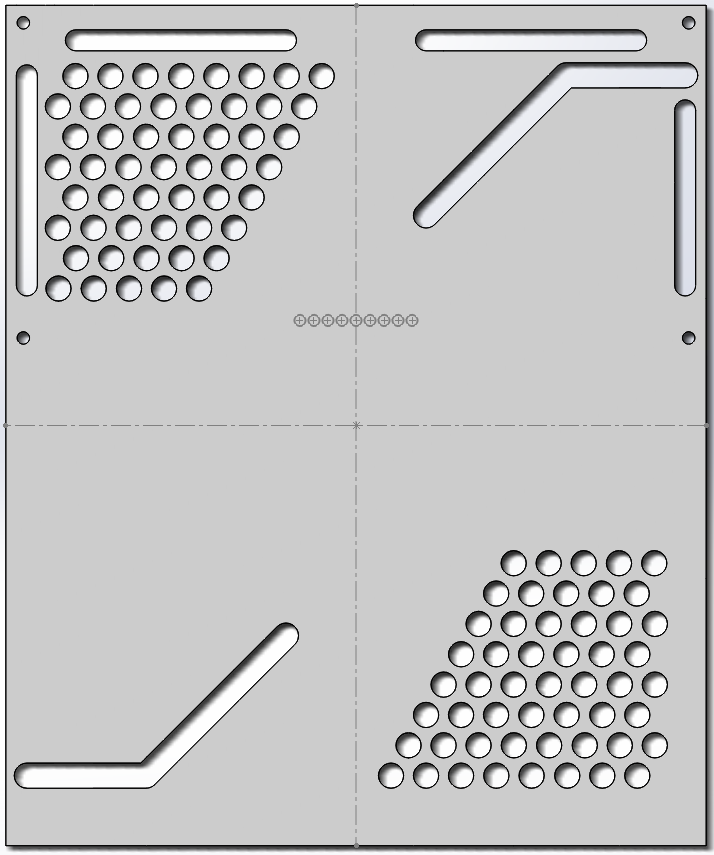
\includegraphics[width = \textwidth]{PR5Images/PlateALTopViewCAD.png}
				\caption{Top view of the aluminum plate.  Note the angled slot in the upper left and bottom right quadrants of the plate as discussed above.  The additional grid of holes was included to allow pedals with only two screws located on adjacent corners (such as the popular Ibanez TS-9) to be accommodated.  The additional vertical and horizontal slots allow the coaxial cables used to connect to the pedal's I/O to pass through the aluminum plate from the circuit board mounted underneath.  The four small holes are for mounting the circuit board.  The row of circles near the center of the piece show the locations of the electrodes used for the hot swapping connector.}
				\label{fig:Plate_AL_top}
			\end{subfigure}
			\begin{subfigure}{0.55\textwidth}
				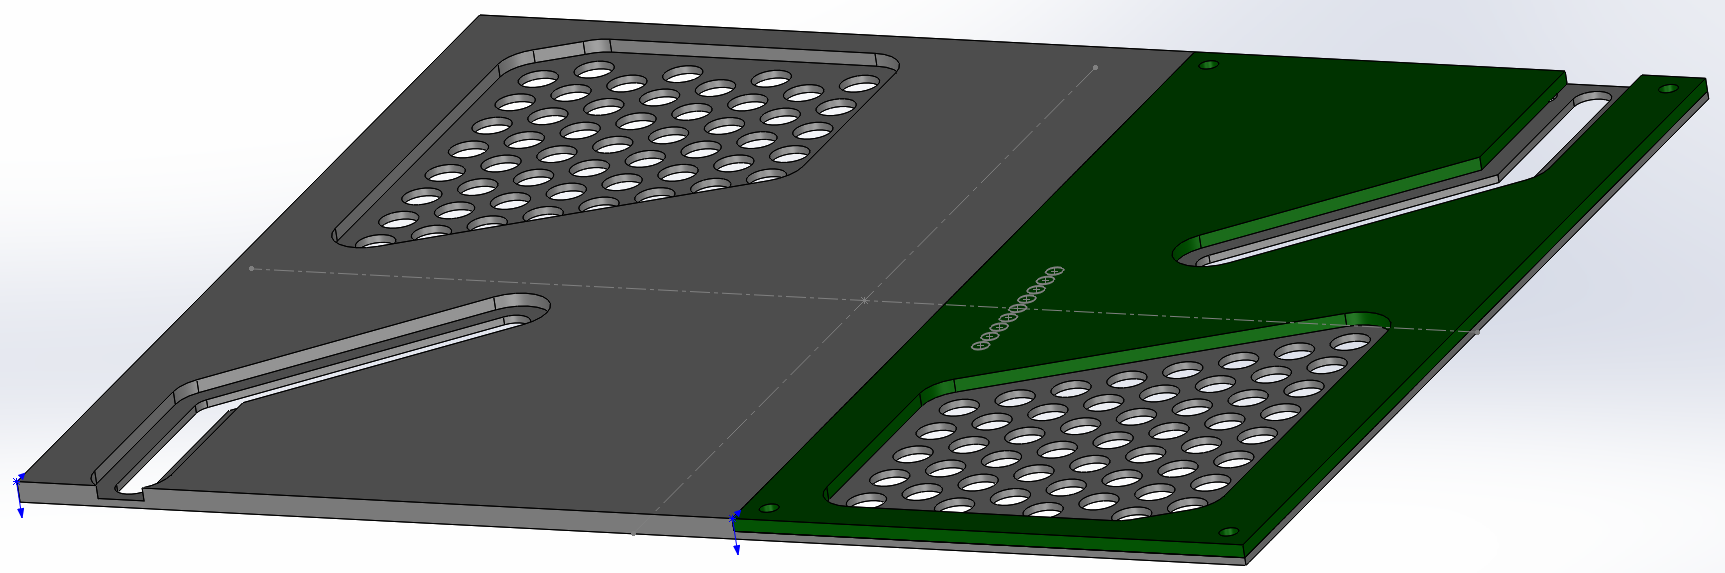
\includegraphics[width = \textwidth]{PR5Images/PlateAsmCAD.png}
				\caption{Assembly view of the plate, with the circuit board shown in green.  Note the pockets in the aluminum allowing the screw heads to catch without needed to waste the full 1/8" of thread length.  A pocket was also cut out for the circuit board to lie flush with the bottom surface.}
				\label{fig:NF_AP_sum}
			\end{subfigure}
			\caption{Universal adapter plate design.}
			\label{fig:finalplatedesign}
		\end{sidewaysfigure}

		The final design of the plate is shown in Figure \ref{fig:finalplatedesign}.  A 5" $\times$ 6" dimension was chosen to allow for room for the I/O connectors and larger pedals.
